\chapter{Практический раздел}

\section{Алгоритм шифрования DES}

\begin{lstlisting}[label=des,caption=Реализация алгоритма шифрования DES]
block_t f(des_t des, block_t r, block_t k) {
    r = e(des, r);

    r = r ^ k;

    block_t b[8];
    for (int i = 8; i > 0; i--) {
        b[i - 1] = r & mask(6);
        r >>= 6;
    }

    for (int i = 8; i > 0; i--) {
        block_t row = get_bit_count_from_right(b[i - 1], 5) << 1 | get_bit_count_from_right(b[i - 1], 0);
        block_t col = (b[i - 1] >> 1) & mask(4);
        b[i - 1] = des.s[i - 1][row][col];
    }

    r = 0;
    for (int i = 1; i <= 8; i++) {
        r <<= 4;
        r |= b[i - 1];
    }

    return p(des, r);
}

void fill_keys(des_t des, block_t k[17], block_t raw_key) {
    k[0] = g(des, raw_key);

    block_t c[17], d[17];
    c[0] = (k[0] >> HALF_KEY_SIZE) & mask(HALF_KEY_SIZE);
    d[0] = k[0] & mask(HALF_KEY_SIZE);

    for (int i = 1; i <= 16; i++) {
        c[i] = cycle_shift_left(c[i-1], HALF_KEY_SIZE, des.shifts[i-1]);
        d[i] = cycle_shift_left(d[i-1], HALF_KEY_SIZE, des.shifts[i-1]);

        k[i] = h(des, d[i] | (c[i] << HALF_KEY_SIZE));
    }
}

block_t des_encrypt(des_t des, block_t t, block_t key) {
    block_t t0 = ip(des, t);

    block_t r[17], l[17];
    r[0] = t0 & mask(HALF_SIZE);
    l[0] = (t0 >> HALF_SIZE) & mask(HALF_SIZE);

    block_t k[17];
    fill_keys(des, k, key);

    for (int i = 1; i <= 16; i++) {
        l[i] = r[i-1];
        r[i] = l[i-1] ^ f(des, r[i-1], k[i]);
    }

    block_t t16 = l[16] | (r[16] << HALF_SIZE);

    return ip_reversed(des, t16);
}

block_t des_decrypt(des_t des, block_t t, block_t key) {
    block_t t16 = ip(des, t);

    block_t r[17], l[17];
    l[16] = t16 & mask(HALF_SIZE);
    r[16] = (t16 >> HALF_SIZE) & mask(HALF_SIZE);

    block_t k[17];
    fill_keys(des, k, key);

    for (int i = 16; i > 0; i--) {
        r[i-1] = l[i];
        l[i-1] = r[i] ^ f(des, l[i], k[i]);
    }

    block_t t0 = r[0] | (l[0] << HALF_SIZE);

    return ip_reversed(des, t0);
}
	\end{lstlisting}

\section{Режим шифрования CBC}
\begin{lstlisting}[label=des,caption=Реализация режима шифрования CBC]
block_t* cbc_encrypt_blocks(block_t* p, int len, block_t key, block_t iv) {
    block_t* c = calloc(len, sizeof(block_t));
    if (c == NULL) {
        return NULL;
    }

    c[0] = des_encrypt(des_default, p[0] ^ iv, key);
    for (int i = 1; i < len; i++) {
        c[i] = des_encrypt(des_default, c[i - 1] ^ p[i], key);
    }

    return c;
}

block_t* cbc_decrypt_blocks(block_t* c, int len, block_t key, block_t iv) {
    block_t* p = calloc(len, sizeof(block_t));
    if (p == NULL) {
        return NULL;
    }

    p[0] = des_decrypt(des_default, c[0], key) ^ iv;
    for (int i = 1; i < len; i++) {
        p[i] = des_decrypt(des_default, c[i], key) ^ c[i-1];
    }

    return p;
}
\end{lstlisting}	


\section{Тестирование}

Корректность алгоритма проверялось путем применения дешифрации на шифрованное сообщение.

Тестирование было проведено на файлах с типами: текстовый (txt), графический (jpeg, png), архив (zip), несуществующий (ubc). Также, был проведен тест с повреждением зашифрованного файла.

В таблице \ref{tbl:test} представлены тестовые данные.

\begin{table}[H]
	\begin{center}
		\centering
		\caption{Тестовые данные}
		\label{tbl:test}
		\begin{tabular}{|c|c|c|} 
			
			\hline
			\multicolumn{1}{|c|}{Номер теста}
			&  \multicolumn{1}{c|}{Тип файла} &  \multicolumn{1}{c|}{Содержимое файла}\\
			\hline
			
			1& txt &  {\specialcell{Наглая Пугачева}} \\ \hline
			
			2& ubc &  $\varnothing$\\ \hline
			
			3& zip & Файлы с тестов 1, 2, 4 \\ \hline
			
			4& png & {\specialcell{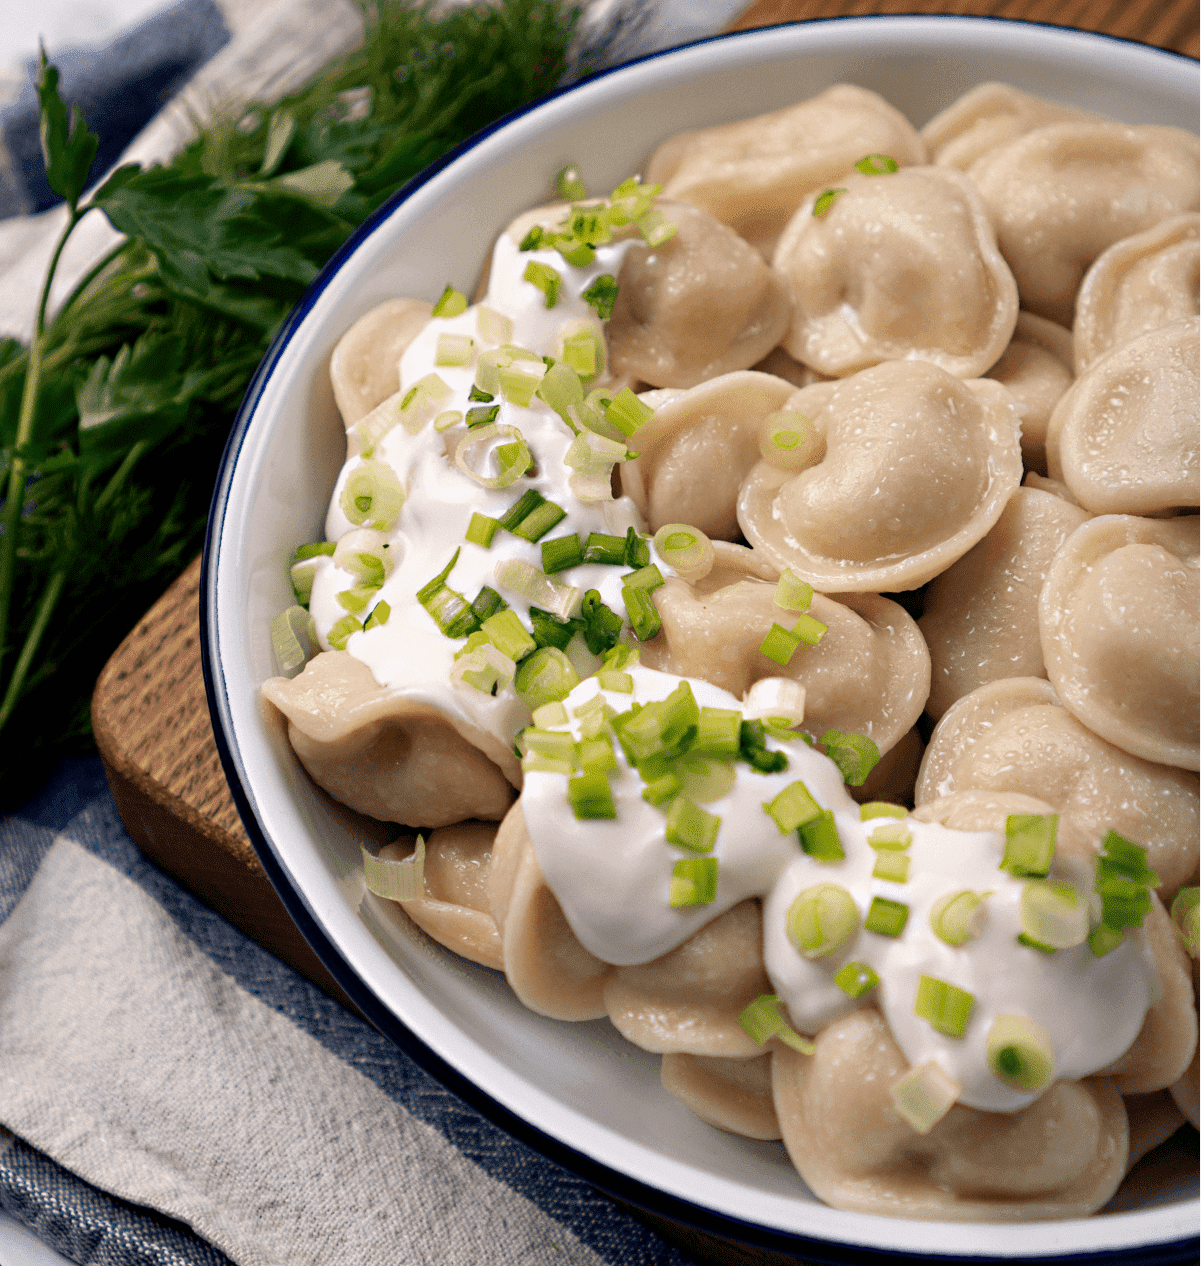
\includegraphics[width=1in]{assets/test4.png}}} \\ \hline
			
			5& jpeg & {\specialcell{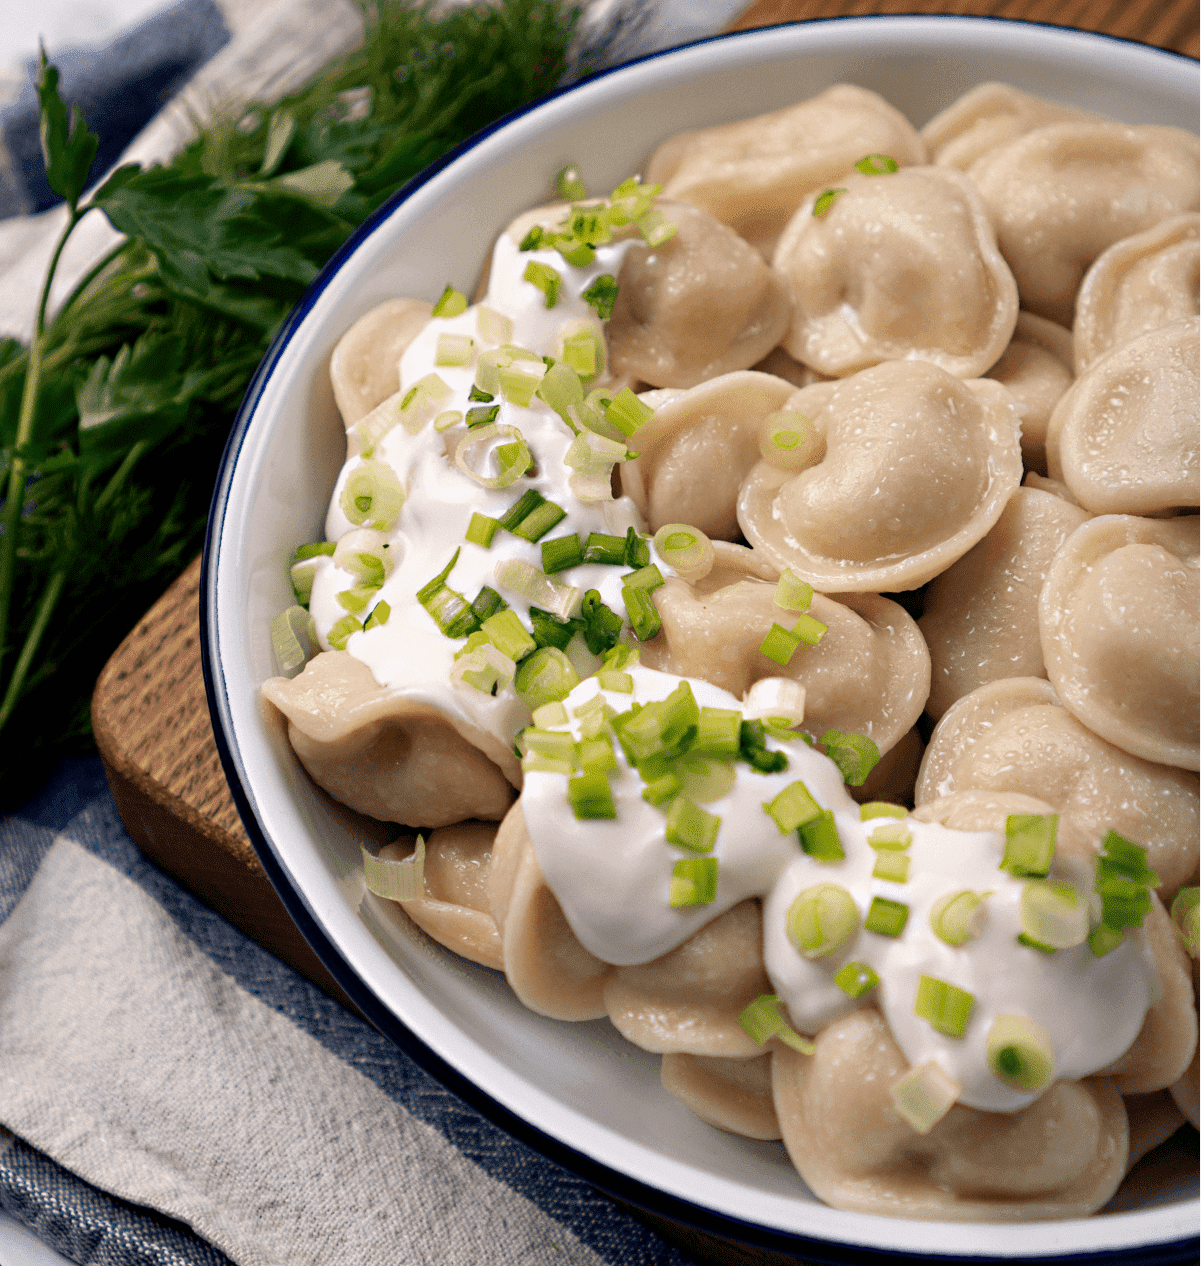
\includegraphics[width=1in]{assets/test4.png}}} \\ \hline
			
			6& {\specialcell{jpeg (corrupted)\\(in english)}} & {\specialcell{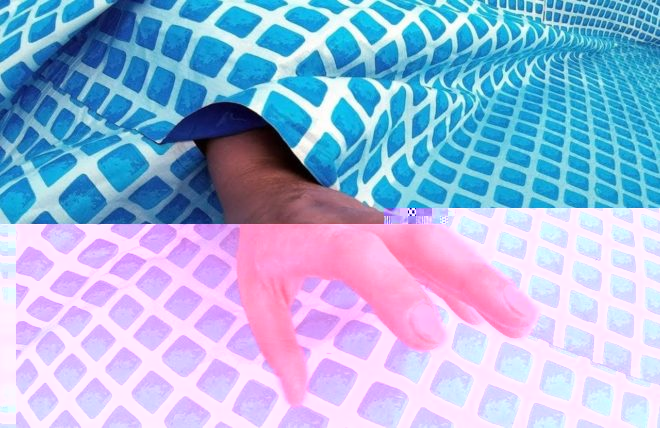
\includegraphics[width=1in]{assets/test6.jpg}}} \\ \hline
			
		\end{tabular}
	\end{center}
\end{table}